\documentclass{proc}

\usepackage{graphicx}
\usepackage{hyperref}
\usepackage{xcolor} 

\begin{document}

\title{Interactive Urban Bike Sharing Visualization}

\author{Sam Longenbach \& Minkun Liu}

\maketitle

\section{Introduction}
Bike sharing systems (BSS) have been becoming a more popular alternative mode of transportation in urban areas.  In general, users are able to checkout a bike from a docking station, ride the bike for a given amount of time, and return it to another docking station. While sharing platforms may differ in cost or max ride time, all docking BSS must always achieve two criteria to meet user demand. First there must always be bikes at all stations and secondly docking stations must not be completely full or a user can not return his or her bike rental. 
 
\noindent There has been a decent amount operations research carried out in the area of tackling the problem of bicycle re-positioning problem \cite{espegren2016static}. The issue of overnight bicycle re-positioning is often viewed as static, while intraday bicycle re-positioning is dynamic as users real-time demand must be accounted for when attempting to balance the system \cite{espegren2016static}. Unsurprisingly the dynamic re-positioning problem is far more challenging than the static re-positioning. In reality in high volume BSS, the re-positioning decisions are made by humans and is not completely automated.       
 
\noindent Existing research in the visualization domain looks to implement a dashboard to highlight bike activity patterns at various stations depending on time of day or types of attraction in close proximity \cite{yan2018visual}. Building off prior research we also look to apply clustering algorithms to highlight stations that behave similarly in regards their demand over the time of day \cite{vogel2011understanding}. For example, BSS stations tend to experience high demand in residential areas during morning during week day hours. We view creating a digestible visualization of station demand as a starting block for a tool that would better inform human decisions in the problem of dynamic bike re-positioning.


\section{Key Takeaway}

Due to the scale of the demand in large bike sharing systems, human are often involved in the problem of bicycle re-positioning. To better inform these decisions we look to create a visualization to allow for better understanding of temporal and spatial features that contribute to particular station demand.

\section{Project Type}

Interactive D3 Visualization

\section{Audience} 

While users and BSS managers could both extract interesting information from our visualization, the intended audience would be managers of BSS. We would like to build off of prior works to create an interactive visualization supplemented with the implementation of clustering algorithms \cite{bargar2014interactive}.
\\~\\
Previous research has shown unsurprisingly that during the weekday in the mornings bicycles are ridden from residential areas to commercial areas and vice versa in the afternoon \cite{bargar2014interactive}. Understanding the natural flows and patterns of the system can lead to BSS managers to make more calculated decisions when it comes to on the fly bicycle re-positioning.        
 
\section{Approach}

\begin{figure*}[t]
  \centering
    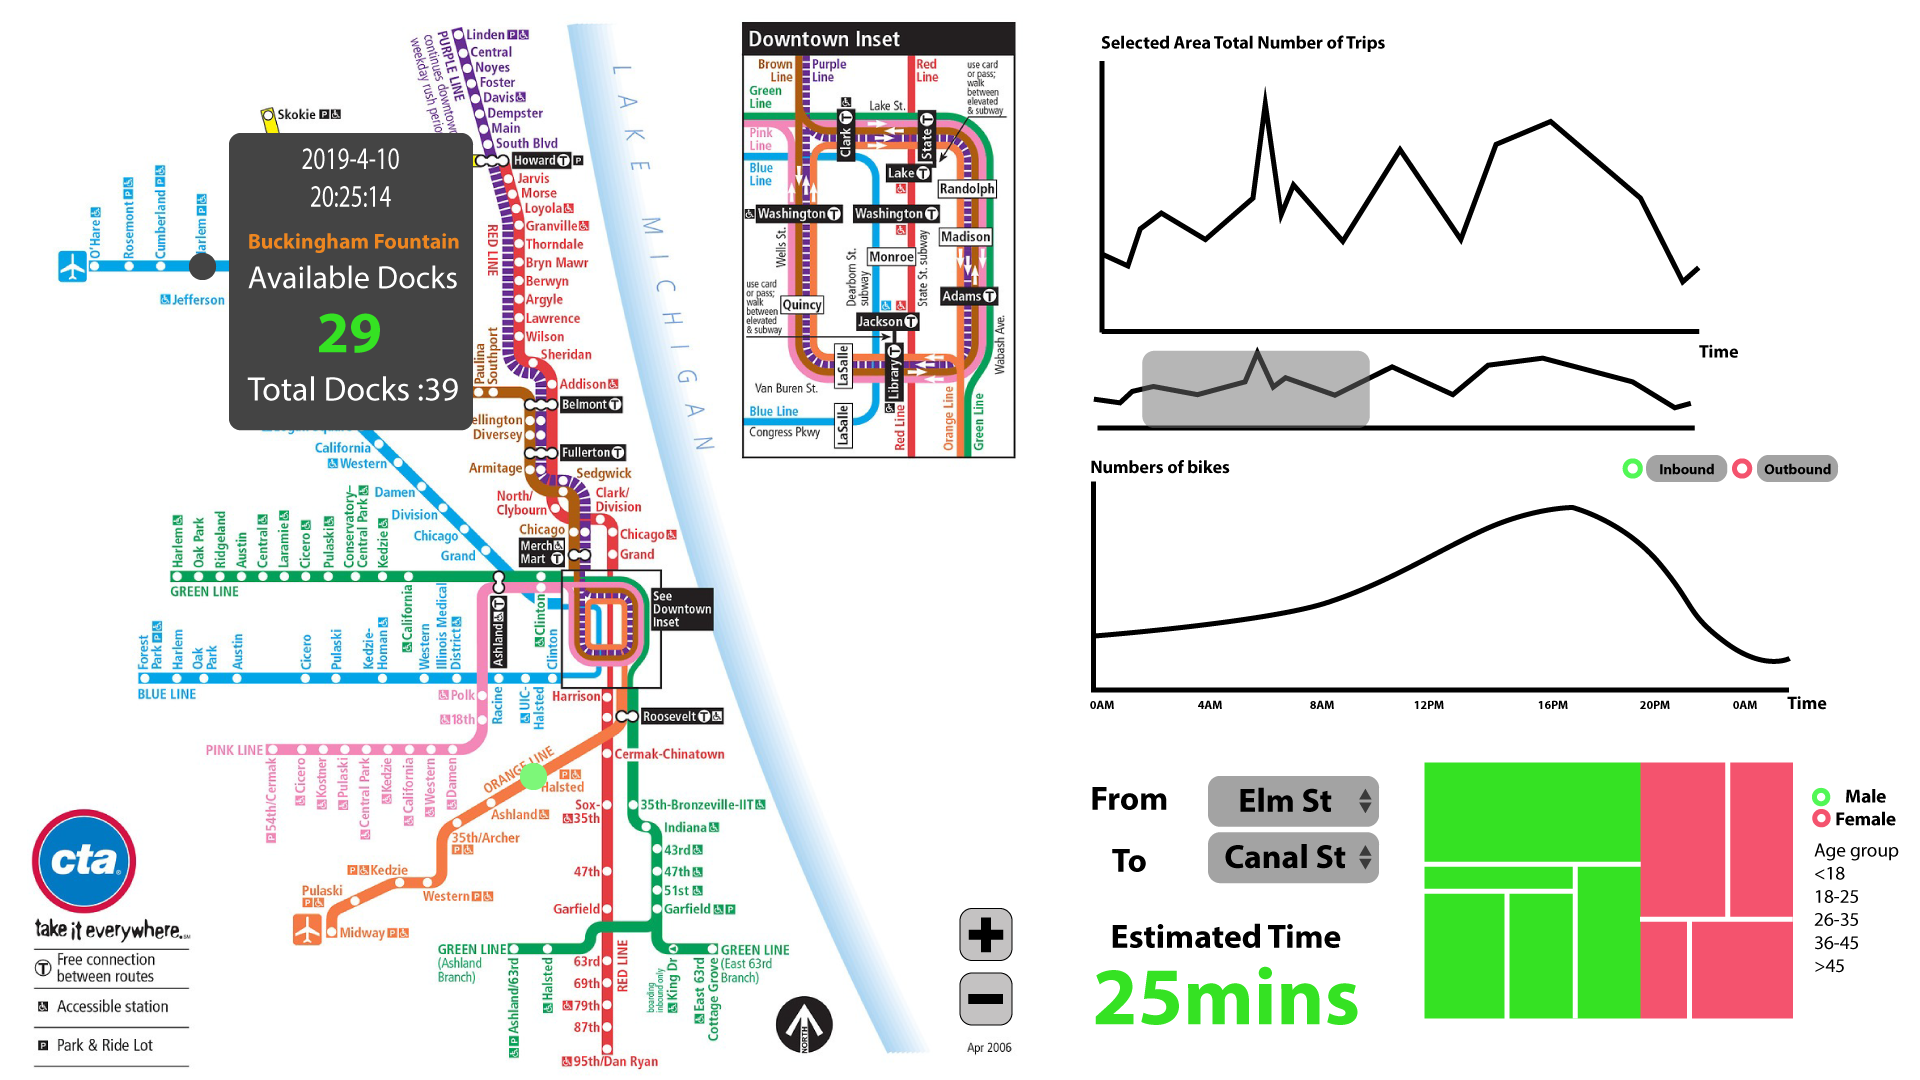
\includegraphics[width=0.9\textwidth]{Sketch}
    \caption{Rough idea of possible interface. \textit{Note that the map is displaying Subway stations in Chicago.} }
  \label{fig:Sketch}
\end{figure*}

In particular we will be working with data from \href{https://www.divvybikes.com/system-data}{\color{blue} Divvy bike share} system located in Chicago. Each row of data contains information on a particular trip. In our case, Divvy provides the start and end time as well as the start and end station. Lastly, if the person is a Divvy member we have additional information of the gender and age of the rider.
\\~\\
\noindent Following in the steps of other research, we plan to preprocess the data in python and calculate the number of outgoing and in going trips from each station in the database. Using a clustering algorithm such as DB-Scan or K-means we can first perform some exploratory analysis on the different stations in the data set. The visual representation has potential to provide useful information on the characteristics of stations. 
\\~\\ 
\noindent Again in align with research we would like to provide some multiple views to provide more information of the users and their trips. To accomplish this we will have to add interactive filter and selection features. However, the extent of these features will be limited by the timeline.    

\section{Best-case Impact Statement}

Provide an informative visualization to inform BSS managers of any temporal or spatial patterns present in their bike station network. We strive to build a graphic so that potential patterns are easily recognizable.   

\section{Major Milestones}

\begin{itemize}

\item Encode the color of stations based on clustering results. 
\item Root the visual encoding of our data in the principles that we have learned in class. 
\item Create interactive map in D3 to show real-time available bikes at station.  
\item As time permits add additional views. For example, estimate the expected travel between stations. 
\end{itemize}

\section{Obstacles}

\begin{itemize}
\item Clustering being unsupervised by nature, it may be difficult to distinctly classify each station. One solution would be to naively classify each station on the spectrum from totally outflowing to totally inflowing of bikes at a given point of time. 
\item Due to limited experience in creating moveable and zoomable maps, more time than initially anticipated may be spent on this portion of the visualization.     
\item While the number of stations in is dataset is approximately 500, the number of trips is around 10 million. We may focus on the most recent years or sample so that are visualization can render in the browser.
\item In order to implement the live status of available bikes we will need to process Python code in on an additional server.     
\end{itemize}

\section{Resources Needed}

\begin{itemize}
\item Python/Pandas to preprocess and aggregate trip data.
\item R or Python to run clustering algorithms to classify stations.
\item Javascript code to build an interactive street map with the location of docking stations.
\item Python code to process \href{https://feeds.divvybikes.com/stations/stations.json}{\color{blue} live JSON feed} of available bikes in the Divvy system.  
\item Javascript code to click on a particular station and update views displaying station specific information. 
\item Continue literature review to inspire our design as we begin to advance with our current design \cite{oliveira2016visual}. 
\end{itemize}

\section{Related Publications}
\begin{itemize}
  \item Bargar explored the utility of building an interactive web-based visual analytics application for comparing usage patterns between bike sharing programs. Utilized the St-DBSCAN algorithm to cluster trips as a way of categorizing flow patterns \cite{bargar2014interactive}. 
  \item Espergren provided an exhaustive literature survey comparing existing models as well as provided a new mathematical formulation for the static bike re-positing problem \cite{espegren2016static}.
  \item Oliveira created pixel-oriented visualization designs that help understand the dynamics of station states and trip circulation patterns \cite{oliveira2016visual}.
  \item Vogel used data mining to gain insight into the complex bike activity patterns at docking stations \cite{vogel2011understanding}.
  \item Yan designed a visual analytics system to interactively explore spatial, temporal, and user dimensions patterns and compared these trends among cities \cite{yan2018visual}.

\end{itemize}

\section{Define Success}

Due to the timeline of this project our main goal is learning. While it may sound cliche, improving our understanding of creating a smooth workable D3 visualization is our main goal. Also figuring out how to process \href{https://feeds.divvybikes.com/stations/stations.json}{\color{blue} live JSON data} is something I would like to learn. Aesthetics and interpretability are very important to us while the processing efficiency is something that will addressed as time permits. 

\bibliographystyle{IEEEannot}
\bibliography{annot}
\end{document}